\documentclass[twocolumn,a4paper]{ltjarticle}

\usepackage{luatexja}
\usepackage{nlp}
\usepackage{amsmath}
\usepackage{graphicx}
\usepackage{scrextend}
\usepackage{setspace}
\usepackage{color}
\usepackage{tabularx}
\usepackage{makecell}

\makeatletter
\let\tti@includegraphics\includegraphics
\renewcommand{\includegraphics}[1]{%
    \tti@includegraphics[width=\linewidth]{#1}}
\makeatother


\title{\textbf{
  パラグラフベクトルとNNによる\\
  文間及びカテゴリ間の関係性を捉えたレーティング予測\\
  Sentiment Classification Reflecting Relation among Sentences and Categories\\
  via Pragraph Vector and Neural Network\\
}}

\author{
  \begin{tabular}{c c c}
    \makecell{外山 洋太\\Yota Toyama}
    & \hspace{4ex}\makecell{三輪 誠\\Makoto Miwa}\hspace{4ex}
    & \makecell{佐々木 裕\\Yutaka Sasaki} \\
    \multicolumn{3}{c}{\makecell{豊田工業大学\\Toyota Technological Institute}}
  \end{tabular}
}
\date{\texttt{\{sd12056, makoto-miwa, yutaka.sasaki\}@toyota-ti.ac.jp}}



\begin{document}

\maketitle

\section{序論}

%企業において商品の評判分析のためのレビューの評判分類は重要な問題である。
%何万件という大量のレビューデータを人手で処理することは難しく、
%計算機による自動化が望まれる。
%その中でレビューを複数のカテゴリにおいて分類する問題がある。
%カテゴリとは、宿泊施設のレビューを例にすると、サービス、立地、食事等の
%レーティングが付けられる各項目のことである。
%しかし、多くの評判分類の手法は一つのカテゴリに対するものである。
%また、この問題に関する従来手法\cite{fujitani15}は、
%文間の関係性を考慮しておらず、
%カテゴリ間については考慮しているものの深い関係性を捉えることができていない。

近年、評判分類において、ニューラルネットワークを用いた手法
\cite{nal14}\cite{rie14}\cite{duyu15}が
提案されており、従来の手法を上回る正答率を達成している。
ニューラルネットワークを分類問題に用いることの利点の一つは
層の数を増やすことによって
入力となる特徴量の深い意味を捉えられることである。
多カテゴリの分類問題に適用すれば、
カテゴリ間の関係性を捉えた分類が実現できる。
さらに、文毎の特徴量を入力とすれば文間の関係性も捉えることができる。

文や文章の意味表現の学習手法として、単語と文章の分散表現を同時に学習する
パラグラフベクトル\cite{quoc14}がある。
これは評判分類問題に対して優れていることが示されている。

本研究は、複数カテゴリにおける評判分類について、
パラグラフベクトル\cite{quoc14}とニューラルネットワークを用いて
文間及びカテゴリ間の関係性を捉えた分類を実現することを目的とする。

提案手法では、パラグラフベクトル\cite{quoc14}によって
生成された各レビューの文書ベクトルと文ベクトルを
ニューラルネットワークによる分類器において分類しレーティング予測を行う。
楽天トラベルのデータセットを用いた実験において、
提案手法は従来手法\cite{fujitani15}に対して2pp以上上回る正答率を
示した。
レーティングの平均二乗誤差(RMSE)を元にした評価基準では、
従来手法\cite{fujitani15}において弱点となっていたカテゴリについて
それを上回る結果を示した。

%ただし、その他のカテゴリでは従来手法\cite{fujitani15}との間に有意な差は
%見られなかった。
%また、パラグラフベクトルが文書と文について適用された場合、
%文書ベクトルと文ベクトルはいくらか異なる特徴を捉えていることが示された。



\section{関連研究}

\subsection{隠れ状態を用いたホテルレビューのレーティング予測}

藤谷ら\cite{fujitani15}は複数のカテゴリにおける評判分類問題に対して、
レビュー内の各文毎に予測した隠れレーティングから
レビュー全体のレーティングを予測する手法を提案している。
文毎のレーティングからレビュー全体のレーティングを予測する際の
カテゴリ間の繋がりを手動で変化させカテゴリ間の関係性を考慮している。
各文の素性にはBag Of Words (BOW)またはn-gramを用いている。
各文毎に隠れレーティングを予測することによって正答率が向上すること、
また、カテゴリ間の繋がりによって正答率が変化することを示している。


\subsection{パラグラフベクトル}

パラグラフベクトルは、文や文章といった大きな単位の言語表現の意味表現を
学習する手法である。これは、Continuous Bag Of Words (CBOW)
またはSkip-gram\cite{yoshua03}という単語の意味表現の学習手法を
応用した手法である。
ここではCBOWを応用したDistributed Memory Model of Paragraph Vectors (PV-DM)
について説明する。

以下に具体的なアルゴリズムを示す。
ここでは文章の意味表現を学習する場合について考える。
学習の概略を図\ref{fig:ParagraphVector}に示す。
まず、意味表現を学習する対象となる文章に含まれる単語を
初めから一つずつ読んでいく。
その際、現在の単語及びその周辺の単語、現在の文章について、
式\ref{eq:ParagraphVector}に示す目的関数$L$を最大化するように
各パラメータの学習を行う。
\begin{gather}
  L = \frac{1}{T} \sum^{T - k}_{t = k} \log p(w_t | w_{t-k}, ..., w_{t+k}),
    \label{eq:ParagraphVector} \\
  p(w_t | w_{t-k}, ..., w_{t+k}) = \frac{e^{y_{w_t}}}{\sum_i e^{y_i}},
    \nonumber \\
  y = b + Uh(w_{t-k}, ..., w_{t+k}, d; W, D) \nonumber
\end{gather}
ここで、$d$は文章、$w_i$は単語、$W$は全ての単語の分散表現を表す行列、
$D$は全ての文章の分散表現を表す行列である。
$k$は片側のウィンドウサイズ、$T$は現在の文章に含まれる単語数である。
ある単語の周辺を表す区間をウィンドウという。
$p$はsoftmax関数により正規化された、文脈から現在の単語が導かれることの
尤度である。
$y$は現在の単語とウィンドウ内の単語及び現在の文章から導出される
正規化されていない対数確率である。
$h(w_{t-k}, ..., w_{t+k}, d; W, D)$は引数となるベクトルを平均したベクトル
または結合したベクトルを返す関数である。

これにより、BOWと異なり、
単語の並び順を考慮した文や文章の分散表現を生成することができる。

\begin{figure}[t]
  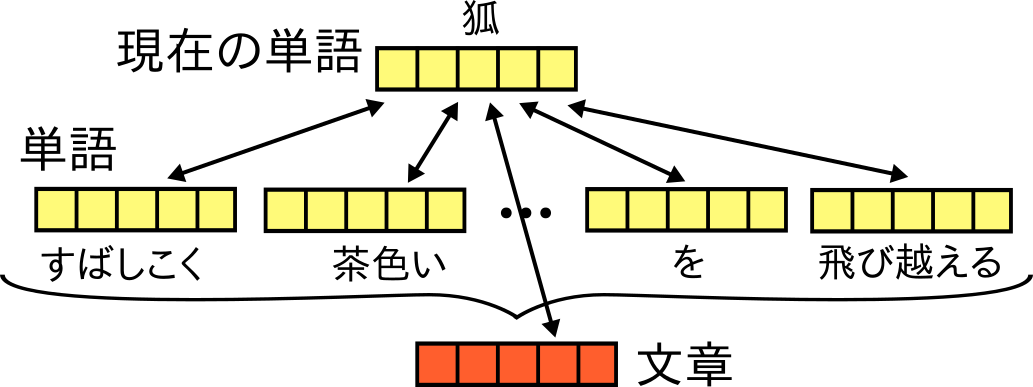
\includegraphics{fig/paragraph_vector.png}
  \caption{パラグラフベクトルの学習の概略}
  \label{fig:ParagraphVector}
\end{figure}


\subsection{ニューラルネットワークを用いた評判分析}

ニューラルネットワークを用いた評判分析の手法が、Nalら\cite{nal14}、
Rieら\cite{rie14}、Duyuら\cite{duyu15}等によって提案されている。

これらの方法に共通するのは、単語の意味表現から畳み込みニューラルネットワークと
全結合ニューラルネットワークを用いて分類を行うことである。
まず、単語の意味表現から畳み込みニューラルネットワークを
用いて単語同士の関係を捉えた特徴量を抽出する。
その後、そこから得られた文書全体の特徴量を
全結合ニューラルネットワークの入力とし多値または二値分類を行う。
また、Duyuら\cite{duyu15}とNalら\cite{nal14}の手法は
ニューラルネットワークのモデルの中にパラメータとして
単語の意味表現を取り込んでいる。これにより、特定の分類問題に対して
それを直に微調整することが可能となる。



\section{提案手法}

提案手法では、PV-DMによってレビュー内の各文及び文章の分散表現を
生成し、それらをニューラルネットワークの入力として分類を行う。

提案するレビュー分類手法の
入力はレビューである文書と正解レーティングの組の集合、
出力は各文書について予測されたカテゴリ毎のクラスである。

初めに、PV-DMを用いて、
各レビューの文書ベクトルとそれに含まれる各文のベクトルを生成する。
文書ベクトルと文ベクトルについては別々に学習し生成する。
式\ref{eq:PVObjective}に示す目的関数$L_d$を最大化するように学習を行う。
\begin{multline}
  L_d = \sum^{T}_{t = n + 1} \{ \log \sigma(s(w_t, w_{t-n}, ..., w_{t-1}, d)) \\
        + \sum^{k}_{w_{t}' \sim P_n}
        \log(1 - \sigma(s(w_{t}', w_{t-n}, ..., w_{t-1}, d))) \},
    \label{eq:PVObjective} \\
\end{multline}
\begin{gather}
  s(w_t, w_{t - n}, ..., w_{t - 1}, d)
    = W_{map}(w_t)
      \cdot \begin{bmatrix} W(w_{t - 1}) \\ \vdots
      \\ W(w_{t - n}) \\ D(d) \end{bmatrix} \nonumber
\end{gather}
ここで、$T$は現在の文章内の単語数、$t$は現在の単語位置、$d$は現在の文章、
$w_i$は位置$i$にある単語、$n$はウィンドウサイズである。
$W(w_i)$は単語$w_i$に相当する単語ベクトルを単語行列$W$から抜き出す関数を表す。
$D(d)$は文章$d$に相当する文章ベクトルを文章行列$D$から抜き出す関数を表す。
関数$s(w_t, w_0, ..., w_n, d)$はある単語とそれが出現する文脈との類似度を
計算する。
行列$W_{map}$は内積によって文脈と単語との類似度を計算するための単語毎
のベクトルを保持する。
文章行列内の各文章ベクトルはレビュー全体を表す文書ベクトル、または、
各レビュー内の文ベクトルを表す。
$\sigma$はシグモイド関数である。
また、式\ref{eq:PVObjective}の中括弧内の右項はネガティブサンプリングを
表す。
ネガティブサンプリングとは、文脈外の単語をデータセットにおける出現確率で
サンプリングし、それらと文脈の意味が遠ざかるように学習する手法である。
$w_{t}' \sim P_n$は文脈外の単語$w_{t}'$を単語の出現頻度$P_n$によって
サンプリングすることを示す。
ただし、出現頻度は極端に頻出する単語の影響を抑えるため
各単語に対して3/4乗している。
現在の単語と同じ単語や同一回の学習で一度サンプリングされた単語は
サンプリングされない。

次に、各レビュー内の全ての文ベクトルに対して重み付け平均を行い、
圧縮された文ベクトルを生成する。
この過程により、各レビューで疎らだった文の数が統一される。
以下に重み付け平均を行う関数を示す。
\begin{gather}
  \mathbf{t}_{i_{sect}} = \sum_{i_{sent}}
                          \frac{w(x_{i_{sect}}(i_{sent}))}
                               {|\sum_{i_{sent}'} w(x_{i_{sect}}(i_{sent}'))|}
                          \mathbf{s}_{i_{sent}}, \nonumber \\
  x_{i_{sect}}(i_{sent}) = \frac{i_{sent} - i_{sect}}{\#sections}, \nonumber \\
  w(x) = \begin{cases}
    \frac{1}{2} (\cos(\pi|x|) + 1) &\text{if $|x| <= 1$} \\
    0 &\text{otherwise}
  \end{cases} \nonumber
\end{gather}
ここで、$i_{sent}$はレビュー内の文のインデックス、
$\#sections$は重み付け平均された後の文ベクトルの数、
$i_{sect}$は重み付け平均された後の文ベクトルのインデックスである。
$s_{i_{sent}}$は文ベクトル、$t_{i_{sect}}$は圧縮された後の文ベクトルである。

次に、レビュー毎の入力を用いて分類器によってレーティング予測を行う。
レビュー毎の入力については後述する。
分類器は全結合ニューラルネットワークによって構成される。
図\ref{fig:MyModel}に各層の結合の様子を示す。

\begin{figure}[t]
  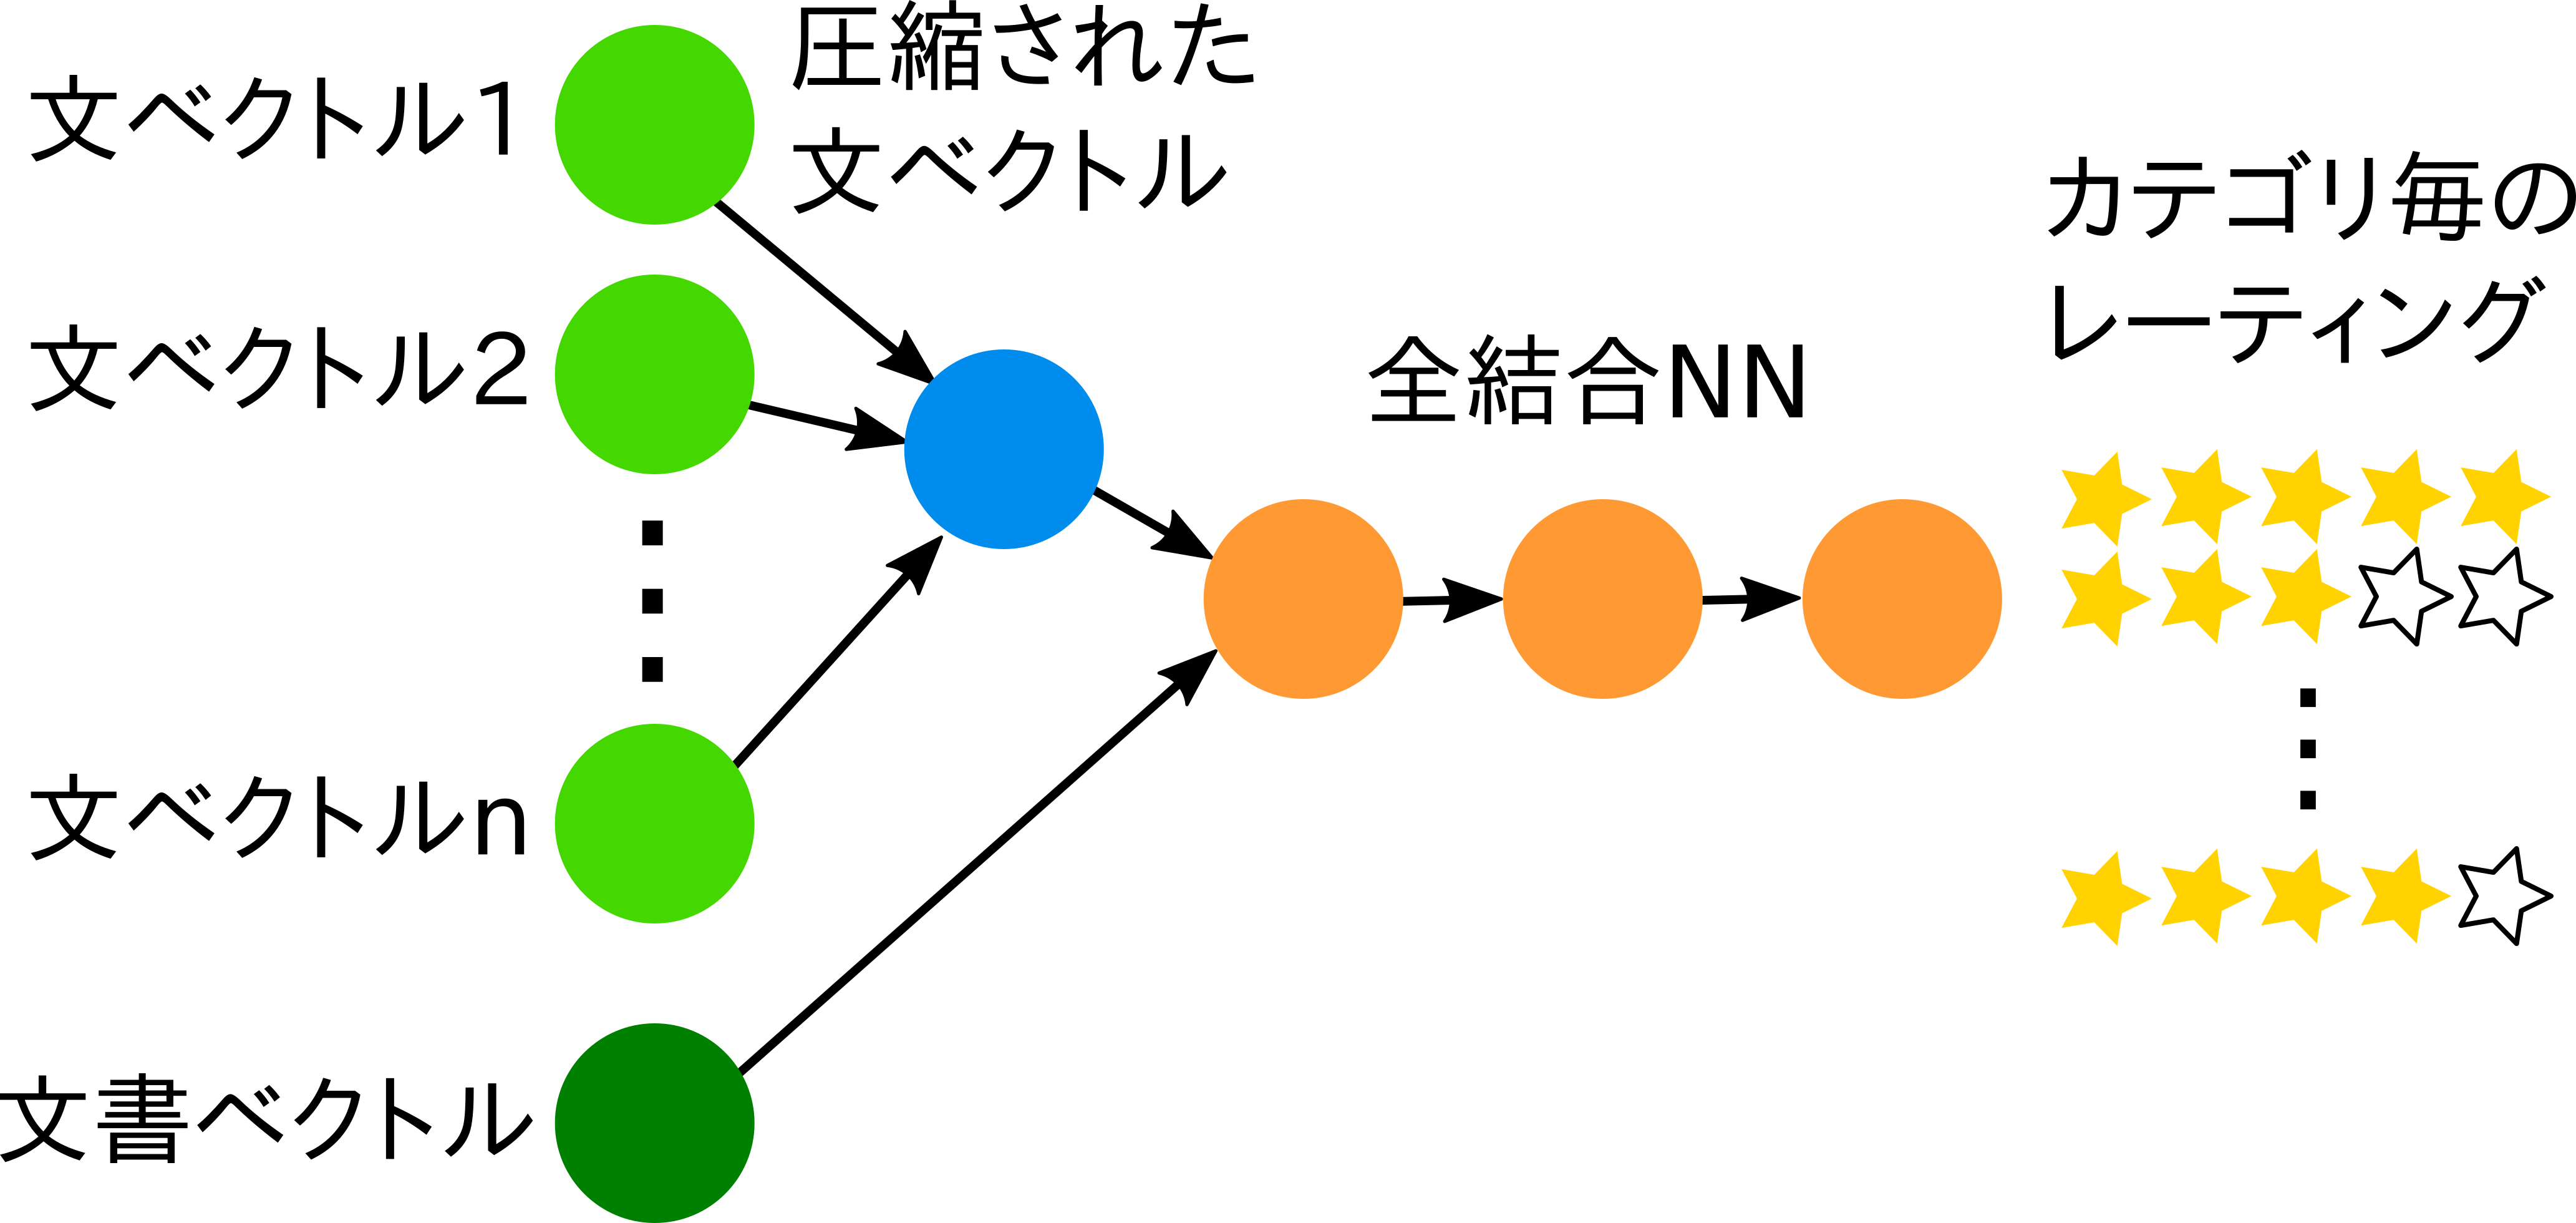
\includegraphics{fig/model.png}
  \caption{全結合ニューラルネットワークによる分類器}
  \label{fig:MyModel}
\end{figure}

ニューラルネットワークの活性化関数には、シグモイド関数を用いる。
また、出力層はカテゴリの数とラベルの数の積だけのユニットを持ち、
各ユニットの出力はあるカテゴリ内であるクラスが選ばれることの
正規化されていない対数確率を表す。
ニューラルネットワークは式\ref{eq:NNObjective}に示す目的関数$E$を
最小化するように学習を行う。
\begin{gather}
  E = - \sum^{N}_{n = 1} \sum^{C}_{c = 1} \sum^{K}_{k = 1}
        d_{nck} \log{y_{ck}(x_n; w)}, \nonumber
  \label{eq:NNObjective} \\
  y_{ck}(x_n; w) = \frac{e^{u_{ck}(x_n; w)}}
                        {\sum^{K}_{j = 1} e^{u_{cj}(x_n; w)}} \nonumber
\end{gather}
各ユニットの出力はカテゴリ毎にソフトマックス交差エントロピー関数によって
損失に変換される。
ここで、$u_{ck}$は出力層のユニットの出力値、$y_{ck}$はカテゴリ$c$において
クラス$k$が選ばれる対数確率、$w$はニューラルネットワークのパラメータである。
$d_{nck}$は$n$番目の文書がカテゴリ$c$でクラス$k$ならば1、
それ以外で0となる値である。
$N$はミニバッチサイズ、$C$はカテゴリの総数、$K$はクラスの総数である。

提案手法としては、Quocら\cite{quoc14}によって提案されている基準手法を拡張し、
NNへの入力となる特徴量が異なる3つの手法を提案する。
基準手法に加え各提案手法に用いられる特徴量を
表\ref{tab:MethodFeatures}に列挙する。

\begin{table}[b]
  \caption{各手法に用いられる特徴量}
  \centering
  \begin{tabularx}{\linewidth}{l | X} \label{tab:MethodFeatures}
    手法 & 特徴量 \\
    \hline
    基準手法 & レビュー全体の文書ベクトル \\
    \hline
    AveSV & レビュー内で平均した文ベクトル \\
    \hline
    WAveSV & レビュー内で重み付け平均によって \\
           & 圧縮された文ベクトル \\
    \hline
    DV-WAveSV & レビュー全体の文書ベクトル、\\
              & レビュー内で重み付け平均によって \\
              & 圧縮された文ベクトル \\
  \end{tabularx}
\end{table}

%AveSVとWAveSVの比較によって、
%文の位置関係が分類に対して重要であるかが示される。
%基準手法とDV-WAveSV、また、WAveSVとDV-WAveSVの基準手法の比較によって、
%文書ベクトルと文ベクトルを同時に特徴量として用いることが
%有効であるかが示される。


\section{実験}

\subsection{実験設定}

提案手法と従来手法\cite{fujitani15}及び基準手法を比較するため、実験を行った。
実験は、各手法の正答率を測定するものと、
その実験で最も正答率の高かった提案手法における予測レーティングと
正解レーティングのRMSEを測定するものの2つを行った。

正答率を測定する実験は基準手法及び3つの各提案手法について行った。
データセットとしては、先行研究\cite{fujitani15}と同様に、
ホテル予約サイト楽天トラベルにおけるレビュー337,266件からレビューの番号順に
訓練データ300,000件、開発データ10,000件、評価データ10,000件を用いた。

レーティングのRMSEを測定する実験は、上記の正答率を測定する
実験で得られた予測レーティングを用いて行った。
正解レーティングが0点であるものは評価から省いている。

表\ref{tab:ParametersOfMethods}に各手法におけるニューラルネットワークの
パラメータ設定を示す。
全ての手法において、中間層の数は1、入力層及び中間層におけるドロップアウト率は
それぞれ0.2と0.5で共通である。
WAveSVとDV-WAveSVにおいて圧縮された文ベクトルの数はそれぞれ3つと2つとした。
全ての実験において文書及び文ベクトルについては、
学習回数は1,024回、学習する単語の範囲は前3単語、単語の最少出現回数は5回、
ベクトルの次元数は600次元に設定し学習したものを用いた。

\begin{table}[b]
  \caption{各手法のパラメータ設定}
  \centering
  \begin{tabular}{l | r r} \label{tab:ParametersOfMethods}
    手法 & 学習回数 & 中間層でのユニット数 \\
    \hline
    基準手法  & 20 & 512 \\
    AveSV & 55 & 256 \\
    WAveSV & 24 & 256 \\
    DV-WAveSV & 30 & 512 \\
  \end{tabular}
\end{table}


\subsection{結果と考察}

表\ref{tab:Accuracies}に正答率を測定する実験の実験結果
及び従来手法\cite{fujitani15}による結果を示す。
表\ref{tab:RMSEs}にRMSEを測定する実験の実験結果を示す。

\begin{table}[b]
  \caption{各手法における正答率}
  \centering
  \begin{tabular}{l | r} \label{tab:Accuracies}
    手法 & 正答率 \\
    \hline
    従来手法\cite{fujitani15}  & 0.4832 \\
    基準手法  & 0.4969 \\
    AveSV & 0.4848 \\
    WAveSV & 0.4866 \\
    DV-WAveSV & \textbf{0.5038} \\
  \end{tabular}
\end{table}

\begin{table}[b]
  \caption{DV-WAveSVと従来手法\cite{fujitani15}におけるレーティングのRMSE}
  \centering
  \begin{tabular}{l | r r} \label{tab:RMSEs}
    手法 & DV-WAveSV & 従来手法\cite{fujitani15} \\
    \hline
    立地      & 0.87 & 0.82 \\
    部屋      & 0.88 & 0.92 \\
    食事      & 2.54 & 3.23 \\
    風呂      & 1.00 & 1.45 \\
    サービス  & 0.85 & 0.85 \\
    設備      & 0.90 & 0.97 \\
    総合      & 0.73 & 0.67 \\
  \end{tabular}
\end{table}

表\ref{tab:Accuracies}より、基準手法と3つの提案手法が全て従来手法の正答率を
上回っている。
DV-WAveSVが従来手法\cite{fujitani15}の正答率を
0.0206上回っていることから、DV-WAveSVが従来手法\cite{fujitani15}より
正答率において優れていることが示されてた。
また、WAveSVの正答率がAveSVの正答率を0.018上回っていることから、
文の位置関係の考慮がレーティング予測に有効であることが示されてた。
さらに、DV-WAveSVが基準手法やWAveSVに比べ高い正答率を示していることから、
文書ベクトルと文ベクトルを同時に特徴量として用いることがレーティング予測に
有効であることが示された。
これは文書ベクトルと文ベクトルがいくらか異なる特徴を学習していることを示す。

表\ref{tab:RMSEs}より、DV-WAveSVは従来手法\cite{fujitani15}が苦手としていた
食事と風呂のカテゴリにおいてそれぞれ0.69及び0.45だけ低い誤差を示した。
藤谷ら\cite{fujitani15}より、本実験で用いたデータセットには、
食事のカテゴリにおいて0点が付与されたレビューが108,079件存在する。
また、風呂のカテゴリでは13,332件、設備のカテゴリでは2,011件存在し、
他のカテゴリでは0件である。
一般に、0点はユーザが何らかの理由でレーティング不可能と判断したことを示す。
よって、DV-WAveSVは従来手法\cite{fujitani15}よりレビュー中の上記のような意味を
よく捉えていると考えられる。
しかし、その他のカテゴリにおいてはDV-WAveSVと従来手法との間に有意な差は
見られなかった。



\section{結論}

本研究では、多カテゴリにおける評判分類問題について、
レビュー全体の文書ベクトルに加えレビュー内の各文ベクトルを用いた
3つの手法を提案した。

実験では、従来手法\cite{fujitani15}及びレビュー全体の文書ベクトルのみを
用いた手法に比べ、文書ベクトルと重み付き平均によって圧縮した
文ベクトルを同時に用いた提案手法が2pp以上高い正答率を示した。
これはレビュー内の文の並びが評判分類に重要であること、及び、
文書ベクトルと文ベクトルがレビューのいくらか異なる特徴を捉えていることを示す。

今後の課題は、文書や文の分散表現を生成する過程を
ニューラルネットワークによる分類器に統合することである。
これによって、学習方法の柔軟性を高めると共にさらなる正答率の向上を目指す。

%今後の課題は、提案手法の中で2つに分かれているモデルの統合である。
%
%提案手法は、分類すべき文書とそれが含む文の分散表現を生成する段階、及び、
%それらを用いて分類を行う段階の2つの段階に分かれている。
%このことは、問題を2つに分けることで個々の問題を単純にしているが、
%同時に文書の分類を一つずつ行うことを難しくしている。
%また、文書や文の分散表現を事前に生成するための
%PV-DMのパラメータは、実際には最大の正答率を達成するため
%分類器のパラメータとして最適化されることが望ましい。
%
%今後は、これらの問題を解決するために、文書や文の分散表現を生成する過程を
%ニューラルネットワークによる分類器に統合する。
%これによって、学習方法の柔軟性を高めると共にさらなる正答率の向上を目指す。




\bibliographystyle{jplain}
\begin{thebibliography}{9}
\bibitem{fujitani15}
  藤谷宣典ら,
  隠れ状態を用いたホテルレビューのレーティング予測.
  言語処理学会第21回年次大会, 2015.
\bibitem{quoc14}
  Quoc Le, and Tomas Mikolov,
  Distributed Representations of Sentences and Documents.
  ICML 2014, 2014.
\bibitem{nal14}
  Nal Kalchbrenner, Edward Grefenstette, and Phil Blunsom,
  A Convolutional Neural Network for Modelling Sentences.
  ACL 2014, 2014.
\bibitem{rie14}
  Rie Johnson, and Tong Zhang,
  Effective Use of Word Order for Text Categorization
  with Convolutional Neural Networks.
  NAACL 2015, 2015.
\bibitem{duyu15}
  Duyu Tang, Bing Qin, and Ting Liu,
  Learning Semantic Representation of Users and Products
  for Document Level Sentiment Classification.
  ACL 2015, 2015.
\bibitem{yoshua03}
  Yoshua Bengio et al,
  A Neural Probabilistic Language Model.
  The Journal of Machine Learning Research 3, 2003.
\end{thebibliography}

\end{document}
